%!TEX TS-program = xelatex
% vim: set fenc=utf-8

% -*- coding: UTF-8; -*-
%!TEX encoding = UTF-8
\documentclass[twoside]{CUGThesis}

\RequirePackage{setspace}
%设置命令
\newcommand{\makestatement}[2][0]{
	\clearpage
	\thispagestyle{empty}
	\vspace*{1em}
	\begin{center}
\begin{spacing}{1.25}{
		\hei \sanhao
		学士学位论文原创性声明
}
\end{spacing}
	\end{center}


\begin{spacing}{1.1}
 \song \xiaosihao

本人郑重声明:所呈交的学位论文是本人在导师指导下独立进行研究工作所取得的研究成果。
除了文中特别加以标注引用的内容外,本论文不包含任何其他个人或集体已经
发表或撰写的成果作品。本人完全意识到本声明的法律后果由本人承担。\\
\end{spacing}

	\begin{spacing}{1}
	\rightline{
	\begin{tabular}{r}
		\\
		作者签名:\hspace{10em}
		 \hspace{4em}年 \hspace{2em} 月 \hspace{2em} 日
	\end{tabular}
	}
	\end{spacing}

	\vspace*{3em}

	\begin{center}
	\begin{spacing}{1.25}{
		\hei \sanhao
		学位论文使用授权书
	}
	\end{spacing}
	\end{center}

\begin{spacing}{1.1}
\song \xiaosihao

本学位论文作者完全了解学校有关保障、使用学位论文的规定,同意学校保留并向有关学位论文管理部门或机构送交论文的复印件和电子版,
允许论文被查阅和借阅。本人授权省级优秀学士学位论文评选机构将本学位论文的全部或部分内容编入有关数据库进行检索,
可以采用影印、缩印或扫描等复制手段保存和汇编本学位论文。\\
\end{spacing}
本学位论文属于
	\begin{enumerate}
		\item 保密 $\Box$,在\uline{\makebox[3em]}年解密后适用本授权书。
		\item 不保密 $\Box$。
	\end{enumerate}
	(请在以上相应方框内打``$\surd$'')

	\begin{spacing}{1}
		\rightline{
		\begin{tabular}{r}
			\\ \\ 
			作者签名:\hspace{10em}
			 \hspace{4em}年 \hspace{2em} 月 \hspace{2em} 日
			 \\ \\  
			 导师签名:\hspace{10em}
			 \hspace{4em}年 \hspace{2em} 月 \hspace{2em} 日
		\end{tabular}
		}
		\end{spacing}
	\vspace{4em}
	\clearpage
}

\include{title}

\title{基于IPv6的HTTP/2过渡应用服务设计与实现} %论文题目
\author{陈立翔} %作者姓名
\date{\today} %日期,默认当日
\school{计算机学院} %院系名称
\classnum{计算机科学与技术} %专业
\stunum {20151001270} %学号
\instructorone{张峰} %指导教师1姓名
\instructoronelevel{副教授}
\instructortwo{陈伟涛} %指导教师2姓名
\instructortwolevel{副教授}

\usepackage{makecell}
\usepackage{multicol}
\usepackage{multirow}
\usepackage{hyperref}

\begin{document}
	\maketitle
	

	\begin{cnabstract}{IPv6 协议;HTTP/2协议;HTTP 网关;反向代理;负载均衡;Go语言;}
		今天,网络早已成为人们生活中不可缺少的部分。同时随着我国网民人口的不断增长,
	互联网环境正在变得愈发复杂。在服务端,开发和运维人员需要利用有限的服务器资源应对更大的并发请求和越来越多的潜在的网络攻击。
	在这种情况下,原有的一些网络协议已经无法满足要求。目前,IPv4的公网地址资源已经枯竭,早在2011年
	亚洲地区就已经无法分配到IPv4地址;而HTTP/1.1协议经过若干次修订后依然被诟病效率过低和功能不足。
	IETF(Internet Engineering Task Force) 发布的 IPv6和HTTP/2协议相关标准已经在很大程度上解决了这些问题,
	如何将旧有的Web应用过渡支持IPv6和HTTP/2是我们目前面临的重要挑战。\par
		本文对于如何让现有的IPv4环境下仅支持HTTP/1.1协议的Web应用能够在IPv4和IPv6双栈环境下工作并
	支持HTTP/2协议,同时尽可能提高服务端的并发性能,开展了以下研究工作:
	\begin{enumerate}
		\item 通过对 Go 语言技术的深入研究,分析其协程和并发模型的技术特点。Go 语言是一门在语言层面
		实现了协程的语言,其实现能够避免操作系统调用产生的开销,单机轻松构建百万级协程,CPU资源的利用率极高,
		是近年来服务端开发中解决高并发问题的重要突破点。
		\item 比较了 RFC 标准中 HTTP/1.1 和 HTTP/2 报文的区别,分析了如何将 HTTP/1.1 的报文加工处理
		成 HTTP/2 的报文。同时结合 Go 语言中原生的 net/http 和 tls 库对报文增加 HTTPS 加密,从而
		兼容目前主流浏览器的实现。
		\item 为了将 HTTP/1.1 应用过渡支持 HTTP/2 ,本文采用 Go 语言技术设计了一个 HTTP 网关。该网关
		通过反向代理技术,在无需对原有应用进行任何修改的情况下,将其升级为支持 HTTP/2 协议,并可在 IPv4和
		IPv6双栈环境下工作。
		\item 基于加权轮询算法和一致性哈希算法对该网关设计了负载均衡策略,
		使得该网关能够支持横向扩容的 Web 应用,应对更复杂的并发情况。
		\item 对该网关进行了压力测试,对比目前市场上提供反向代理功能的服务器如 Apache, Nginx 等,
		得出该网关在一些情况下能够提高系统并发数和减少响应时间,提升用户体验。并通过火焰图分析该网关在
		实际工作环境中的性能瓶颈。
	\end{enumerate}
		\par
		综上所述,本文设计的基于 Go 语言的 HTTP 反向代理网关,能够作为在IPv4和IPv6双栈环境下的 HTTP/2 过渡应用,
	并且具有较好的并发性能。经过测试,具有一定实用价值。
	\end{cnabstract}
	
	\begin{enabstract}{IPv6 Protocol; HTTP/2 Protocol; HTTP Gateway; Reverse Proxy; Load Balancing; The Go Programming Language;}
		The Internet has become an indispensable part of people's lives nowadays.
		At the same time, with the growth of the netizen population in China, the Internet 
		environment is becoming more and more complicated. On the server side, development and operations
		personnel need to use limited server resouces to handle larger concurrent requests and more 
		pontential network attacks. In this case, some of the old network protocols are not 
		sufficient enough. At present, hte public network address resources of IPv4 have been
		exhausted. As early as 2011, the Asian region has been unable to allocate IPv4 addresses; 
		and the HTTP/1.1 protocol has been criticized for being inefficient and short of functions
		 after serveral revisions. IETF(Internet Engineering Task Force) had published IPv6 and HTTP/2 protocol and it had largely solved 
		 these problems.\par 
		 This article describes how to enable the Web application that supports only the HTTP/1.x protocol
		 in the existing IPv4 environment to work in the IPv4 and IPv6 dual-stack environment and support 
		 the HTTP/2 protocol, while improving the concurrent performance of the server as much as possible. research work: \par 
		 \begin{enumerate}
			\item  Through the in-depth study of Go (programming language) technology, analyze the technical characteristics of its coroutine and concurrency model. 
			Go is a language that implements coroutine at the language level. Its implementation can avoid the overhead caused by operating system calls. 
			It is easy to build a million-level coroutine in a single machine. The utilization of CPU resources is extremely high. An important breakthrough to address high concurrency issues.
			\item Compare the difference between HTTP/1.1 and HTTP/2 messages in the RFC standard, and analyze how to process HTTP/1.1 messages into HTTP/2 messages. At the same time, 
			it combines the native net/http and tls libraries in the Go language to add HTTPS encryption to the message, which is compatible with the current mainstream browser implementation.
			\item  Based on the weighted round-robin algorithm and the consistent hash algorithm, a load balancing strategy is designed for the gateway, which enables the gateway to support
			 horizontally expanded Web applications and cope with more complex concurrency situations.
			 \item Test the gateway. Compared with the servers that provide reverse proxy functions on the market, such as Apache, Nginx, etc., it can be concluded
			  that the gateway can improve the number of concurrent systems and reduce response time in some cases, improving the user experience. The performance of the gateway
			   in the actual working environment is analyzed through the flame graph.
		 \end{enumerate}
		 \par
		 In summary, the Go-based HTTP reverse proxy gateway designed in this paper can be used as an HTTP/2 transition application in IPv4 and IPv6 dual-stack environments, and has good concurrency
		  performance. After testing, it has certain practical value.
	\end{enabstract}
	
	\makeToc
	
	%---------------------------------------------开始正文---------------------------------------------
	
	%--------------------------------------------- 第一章 ---------------------------------------------
	\begin{spacing}{2}
		\section{绪论}
	\end{spacing}
	\subsection{研究背景及其意义}
	各种网络协议常常被称为互联网时代的基石。随着网络环境的变化,网络协议也需要适应时代的需求
	迭代升级。\par
	从1996年开始,一系列关于IPv6协议的RFC标准发表出来,旨在取代原有的IPv4协议。IPv6的地址长度为
	128位,能提供远多于IPv4 的地址数量。在IPv6环境下,将不需要IPv4环境下为了解决地址数量不足而衍生出的NAT等技术,每个设备都能得到
	一个公网IP,有利于物联网等技术的发展。但IPv6技术的推进还需要一段时间,在未来一段时间内我们都将
	面临着IPv4和IPv6共存的互联网环境。\par
		2015年发布的HTTP/2协议则旨在取代HTTP/1.x协议。为了提高网络传输的效率,更有效地利用网络资源,
	该协议增加了二进制分帧,多路复用和头部压缩等新的特性。同时目前浏览器中 HTTP/2 
	实现都强制要求数据通过 HTTPS 加密,而不是像 HTTP/1.x 协议那样
	将数据明文发送。这显著增强了数据传输的安全性,有效避免数据被劫持等安全隐患。\par
	将现有的应用迁移升级到这些新协议上将会是一个漫长且耗资巨大的过程。如何在今天这种多种协议共存的情况下,
	将旧有的应用以尽可能低的成本过渡迁移到新协议上,且具有较好的性能?\par
		目前国内外最广泛使用的HTTP服务器Apache和Nginx都支持反向代理并升级IPv6和HTTP/2协议的功能。
		通过配置都可以支持通过反向代理将旧有的服务升级至支持IPv6和HTTP/2协议。

	\subsection{国内外相关工作介绍}
	目前国内外市场上90\%以上的反向代理HTTP网关服务器为Apache 和 Nginx。这两者都基于C语言编写。也有很多人对这些网关进行了二次开发,例如中国工程师章亦春等人基于Nginx开发的OpenResty\cite{OpenResty}等。\par
	这些网关在不断的迭代过程中也陆续加入了IPv6和HTTP/2协议的支持。它们由于久经实际生产环境考验,具有较强的稳定性。
	但由于一些历史遗留原因,也或多或少存在诸如开发效率较低,并发能力较差等问题。
	\subsubsection{Apache}
	Apache HTTP Server (简称Apache)是 Apache 软件基金会维护开发的一个开源HTTP服务器软件。它自1995年诞生以来,
	一直是世界上最被广泛使用的HTTP Server。同时其也提供反向代理功能,并已加入 HTTP/2 和 IPv6 的支持。\par 
	Apache在二十多年间已迭代数个版本,具有极佳的稳定性和大量的插件,能够帮助开发者快速构建小型Web应用。\par
	但是 Apache 在应对并发请求时,使用的是传统上基于进程或线程模型架构,通过多线程来处理并发请求。
	事实上这种模型虽然稳定,却无法发挥出现代计算机的性能,后面在讨论Go语言的并发模型时将会谈到这一点。\par
	\subsubsection{Nginx}
	Nginx是俄罗斯工程师Igor Sysoev在2004年发布的一款异步框架的高性能HTTP服务器,常被用作反向代理和负载均衡器。
	目前绝大多数高并发量的网站都使用Nginx作为HTTP服务器。它在不断的迭代中也陆续加入了IPv6和HTTP/2的支持。\par
	Nginx的出现就是为了解决Apache的并发模型无法解决的C10K问题。C10K指的是能够使单机服务器承受一万以上的并发连接请求。
	Nginx创造性地将模块化加入了设计之中,非常方便于二次开发。如由中国工程师章亦春等人开发的OpenResty,
	阿里巴巴公司开发的Tengine都是根据实际需求基于Nginx二次开发的HTTP服务器。\par
	Nginx采用了epoll多路复用机制来应对高并发请求。epoll是Linux 2.6版本内核之后加入的特性。
	Linux提供了三种I/O多路复用模型,select, poll 和 epoll。它们分别是基于数组,链表和哈希表保存文件描述符的
	I/O多路复用模型。显然2.6版本加入的epoll模型所使用的哈希表具有最低的时间复杂度,
	这可以大大减少操作系统切换上下文的开销,应对高并发连接。根据官方的测试结果,在理想情况下,Nginx单机
	可以应对五万个并发连接,而在实际的运作中,可以支持二万至四万个连接。\par 
	但是这也给Nginx带来了一个问题.在非Linux系统下,无法使用这些操作系统底层的API来进行I/O多路复用,这时
	其并发性能会大大下降。对于情况较为复杂的跨平台服务端解决方案来说,Nginx并不合适。\par
	\subsection{论文主要工作和章节结构}
	本文主要针对如何在IPv4和IPv6双栈环境下将旧有的HTTP/1.x的Web服务过渡升级支持HTTP/2设计了一个
	网关。该网关通过反向代理的形式升级协议。并且该网关具有高并发和易跨平台的特性,避免了上述解决方案的一些缺点。\par 
	论文的内容和章节结构如下:
	\begin{enumerate}
		\item 第一章:绪论。主要介绍了研究背景,以及通过反向代理升级IPv6和HTTP/2协议的这方面国内外的
		一些成熟解决方案及其存在的问题,以及本文主要工作安排。
		\item 第二章:Go 语言服务端相关技术介绍。简单介绍了Go语言的背景和一些内置库实现,并分析了其并发模型,
		说明了Go语言应用在本项目的一些优势。
		\item 第三章:HTTP/1.x 到 HTTP/2 的转换实现。深入分析了RFC标准中 HTTP/1.x 协议和 HTTP/2 协议的
		差异,根据这些差异拟定了程序中通过怎样的流程去升级HTTP协议。同时也对广泛使用的Websocket协议做了处理。
		\item 第四章:IPv4 和 IPv6 双栈环境下反向代理功能的实现。介绍了本设计的核心功能,反向代理功能是如何
		实现的,以及程序如何在IPv4和IPv6双栈环境下工作。并介绍了通过加权轮询算法和一致性哈希两种算法设计的两种负载均衡策略。
		\item 第五章:性能分析。通过压力测试和火焰图两种形式对本设计的性能进行了分析。
		\item 第六章:总结和展望。总结了本设计的功能、特性和缺点,阐述了一些辄需改进的地方。
	\end{enumerate}
	
	%------------------------------------------- 第二章 ---------------------------------------------
	\begin{spacing}{2}
		\section{Go语言相关技术介绍}
	\end{spacing}
	\subsection{Go语言简介}
	Go语言(简称Go)是由美国谷歌(Google)公司发布的一种静态强类型、编译型、并发型并具有垃圾回收功能的编程语言\cite{donovan2015go},于2009年推出最初版本并开源。
	其作者 Rob Pike 和 Ken Thompson 等人均曾经在美国贝尔实验室工作,参与了C语言和Unix系统的开发工作。\par 
	Go的发明是为了解决C/C++在服务端开发时的一些问题。在面向高并发环境的程序开发时,C++由于其过多的语言特性,导致程序员对语言的学习成本极高;C语言则恰好相反,过于简单的语言特性和较低的抽象层次,使得编写代码本身就十分复杂。
	同时它们较为落后的包管理机制不利于对代码的高效复用。依赖于系统底层API的网络操作等也使得其跨平台能力不强。\par
	Go本身语法大量借鉴了C语言,并简化了一些部分,其关键字数量比C语言还要更少。对于有一定C语言开发经验的开发者来说学习成本较低。
	Go内置大量网络编程相关的库,可以大大简化网络编程的工作,更重要的是,其实现不依赖于任何操作系统底层API,
	这使得Go编写的程序可以较为容易地交叉编译并在多平台运行。\par
	Go也在一定程度上支持一些面向对象编程的方法。其程序以包的形式组织,包实质上是一个包含Go文件的文件夹。包内的代码共享相同的命名空间,为区分包内
	包外的私有成员,Go将以大写字母开头的对象(包括函数,变量等)对其它包可见,其它的则不可见。\par 
	\subsection{Go语言的并发模型}
	Go语言最为重要的特性来源于其在语言层面对并发的支持。这里讨论的是 Go 1.7 版本及之前的经典并发模型。
	虽然在后期版本增加了一些新的功能或语法糖,但本质上还是离不开我们后面讨论的这些并发模型。
	\subsubsection{协程(Coroutine)}
	我们知道,线程和进程都是在操作系统层面上实现的。相对于进程来说,线程可以减少调用时的上下文开销,具有更小的颗粒度。\par 
	但是对于服务端接受HTTP请求这样的需求来说,线程的粒度依然过大。对每个请求或TCP连接开一个线程来处理的话,
	会有大量的I/O阻塞占用CPU时间,造成资源的极大浪费。\par 
	Go在语言层面上实现了协程,通过关键字go来进行调用。协程拥有自己的Runtime,每个协程都有自己的堆栈,
	Go封装了自己的一套协程调用方法,实际还是通过线程来执行任务。Go 的协程在理想状态下可以达到百万级并发\cite{deshpande2012analysis}。
	\subsubsection{通道(Channel)}
	协程是在语言层面上实现的,因此我们不能使用操作系统中实现的诸如信号量这样的API对其做并发操作。Go语言
	是在语言层面上实现了一种称之为通道(Channel)的数据结构,来进行协程间通信的操作。\par 
	Channel本质上是一个先进先出队列(FIFO),协程内可以通过select关键字监听Channel中是否有元素可以做
	出队操作,当Channel中没有元素时协程阻塞。协程中同样也可以对Channel直接做写入操作,当队列满时也发生阻塞。
	通过这样的机制就能实现协程之间的通信。
	\subsubsection{上下文(Context)}
	上下文(Context) 在与 API 和慢处理交互时可以派上用场,特别是在生产级的 Web 服务中。\par 
	Context实现的主要功能为在协程之间共享状态变量,和在被调用的协程外部,通过设置ctx变量值,将“过期或撤销这些信号”传递给“被调用的程序单元”。
在网络编程中,若存在A调用B的API, B再调用C的API,若A调用B取消,那也要取消B调用C,通过在A、B、C的API调用之间传递Context,以及判断其状态,就能解决此问题。

	
	
	%--------------------------------------------- 第三章 ---------------------------------------------
	\begin{spacing}{2}
		\section{HTTP/1.1到HTTP/2的转换实现}
	\end{spacing}
	要想实现HTTP/1.1到HTTP/2的转换,我们首先要了解这两个协议的特性及其异同,针对性地设计转换的方法。\par
	世界上最早的HTTP协议标准源于1991年发布的HTTP/0.9标准。该版本及其简单,只有一个HTTP方法 GET。它具有
	以下特点:
	\begin{itemize}
		\item 客户端/服务端响应都是ASCII字符
		\item 客户端请求由一个回车符(CRLF)结尾
		\item 服务器响应的是超文本标记语言(HTML)
		\item TCP连接在文档传输完毕后断开
	\end{itemize}
	\par
	显然这个协议是十分简陋的。它无法处理用户登录等稍微复杂一点的操作,以及各种富文本。1996年IETF发布了正式的HTTP/1.0标准,
	相较于之前的版本它有一些明显的特性:
	\begin{itemize}
		\item 服务端响应增加了响应状态
		\item 请求和响应增加了多行首部
		\item 响应内容不再局限于HTML
	\end{itemize}
	\par
	HTTP/1.0依然存在很多问题和值得优化的地方。比如对TCP连接的复用,大文件传输的优化,浏览器缓存较差等等。
	1999年发布的HTTP/1.1就是为了解决这些问题的。该协议一直到2014年,依然在不断地进行修订。它具有以下
	几个显著特性:
	\begin{itemize}
		\item 持久连接(Keep-Alive机制)
		\item 传输编码(Chunk机制)
		\item 字节范围请求(Accept-Ranges)
		\item 增强的缓存机制(协商缓存和强缓存)
	\end{itemize}
	\par
	HTTP/1.1已经有二十年的历史,并且依然在被广泛使用,十分稳定。但2015年,IEFT依然发布了HTTP/2用于取代
	HTTP/1.1。这源于互联网快速的发展,使得其无法适应当前的需求。\par 
	本章介绍HTTP/1.1存在的问题,HTTP/2的新增特性和在Go语言下将HTTP/1.1报文转换为HTTP/2的方法。以及浏览器和
	服务端之间协议的协商机制和对目前广泛存在的WebSocket协议的处理。

	\subsection{HTTP/1.1的困境}
	如今的Web应用已经大大超出了人们在最开始对Web的想像。在早期,一个网站往往只有一个简单的HTML页面。
	但是在今天,任意一个门户网站都有大量的流媒体,AJAX请求,图片……人们也不再仅仅使用PC来浏览网页,
	移动端和物联网设备逐渐成为了主流。这种情况下,一个Web页面中的HTTP请求数和网站所占用的通信和存储空间会大大增加。
	httparchive.org对目前互联网的的大量网站做了监测,结果如图所示\cite{httparchive}。\\ 
	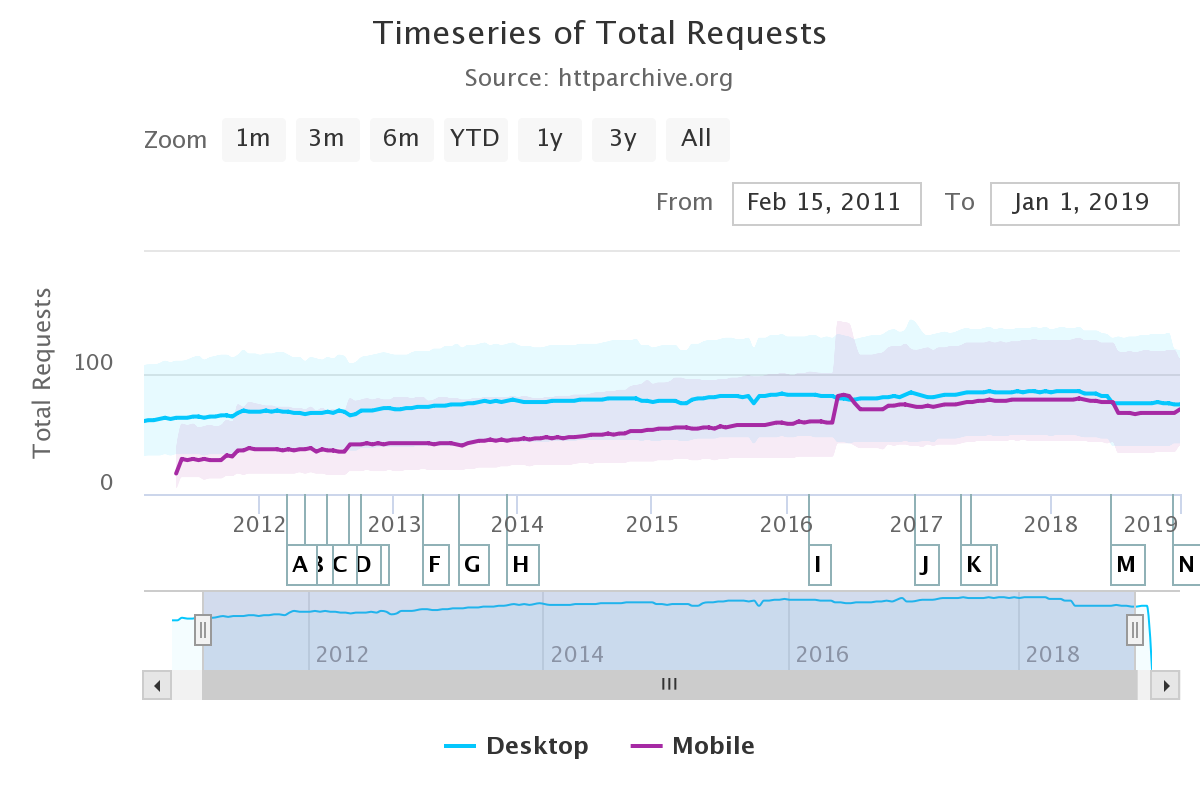
\includegraphics[scale=0.31]{Figures/web_total_reqs.png}\\
	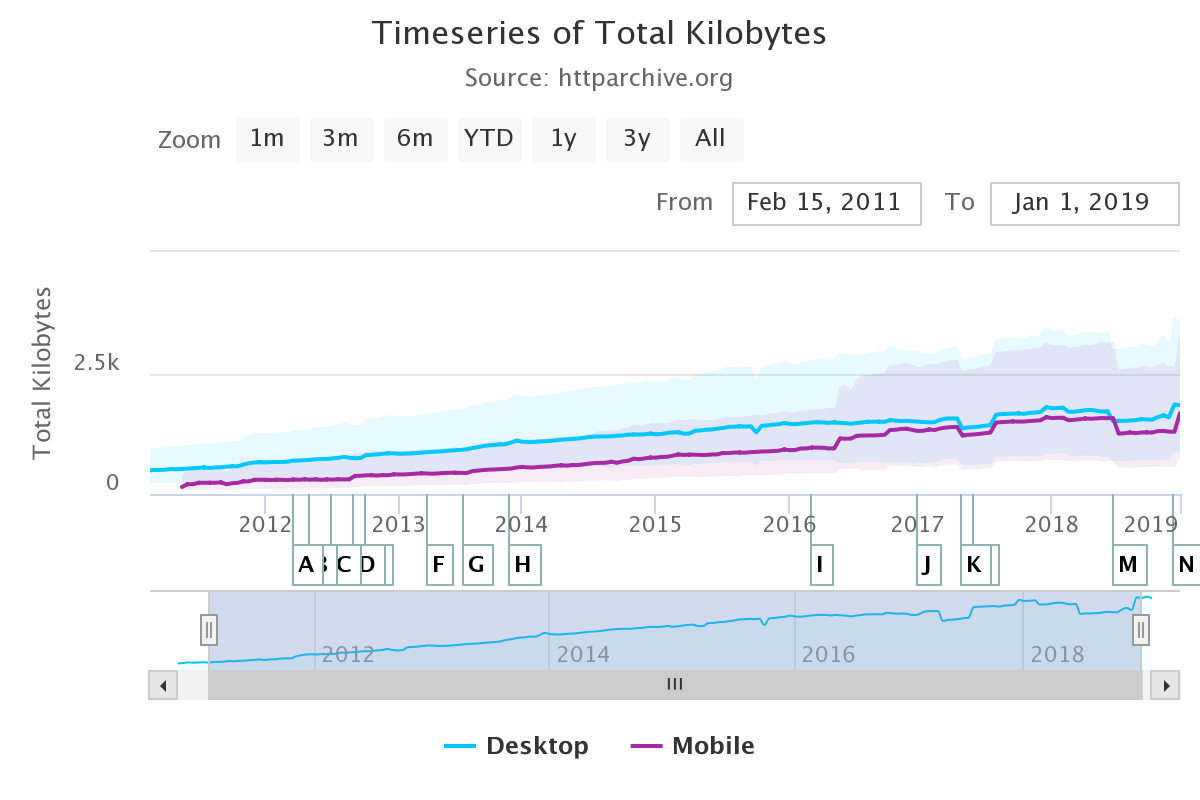
\includegraphics[scale=0.31]{Figures/web_total_size.png}\\
	\par 
	从图中可以看出,随着时间的推移,浏览一个网站平均需要的HTTP请求数量和资源的大小都在稳步上升。
	目前在没有缓存的情况下,在PC端浏览每个网站平均需要下载2000kb以上的资源,发生70个以上的HTTP请求。在
	移动端这个数字还要更高。这给了网络传输以很大的挑战。事实上,
	用户浏览网站时,在等待的过程中,平均有69.5\%的时间是耗费在网络操作的阻塞上的。\par 
	而HTTP/1.1协议本身对并发连接并没有做很好的优化。Keep-Alive机制本身只能复用连接,但是对并发连接并没有什么帮助。
	早期的标准RFC2616甚至规定浏览器中同域名只能有两个连接\cite{fielding2006hypertext}。
	RFC7230虽然去掉了这一限制,但现代浏览器中依然限制同域最多只能有6个并发连接。在浏览器中打开一个HTTP/1.1的网站,
	我们很容易在控制台中看到网络资源的加载时序,如图所示。\\ \par 
	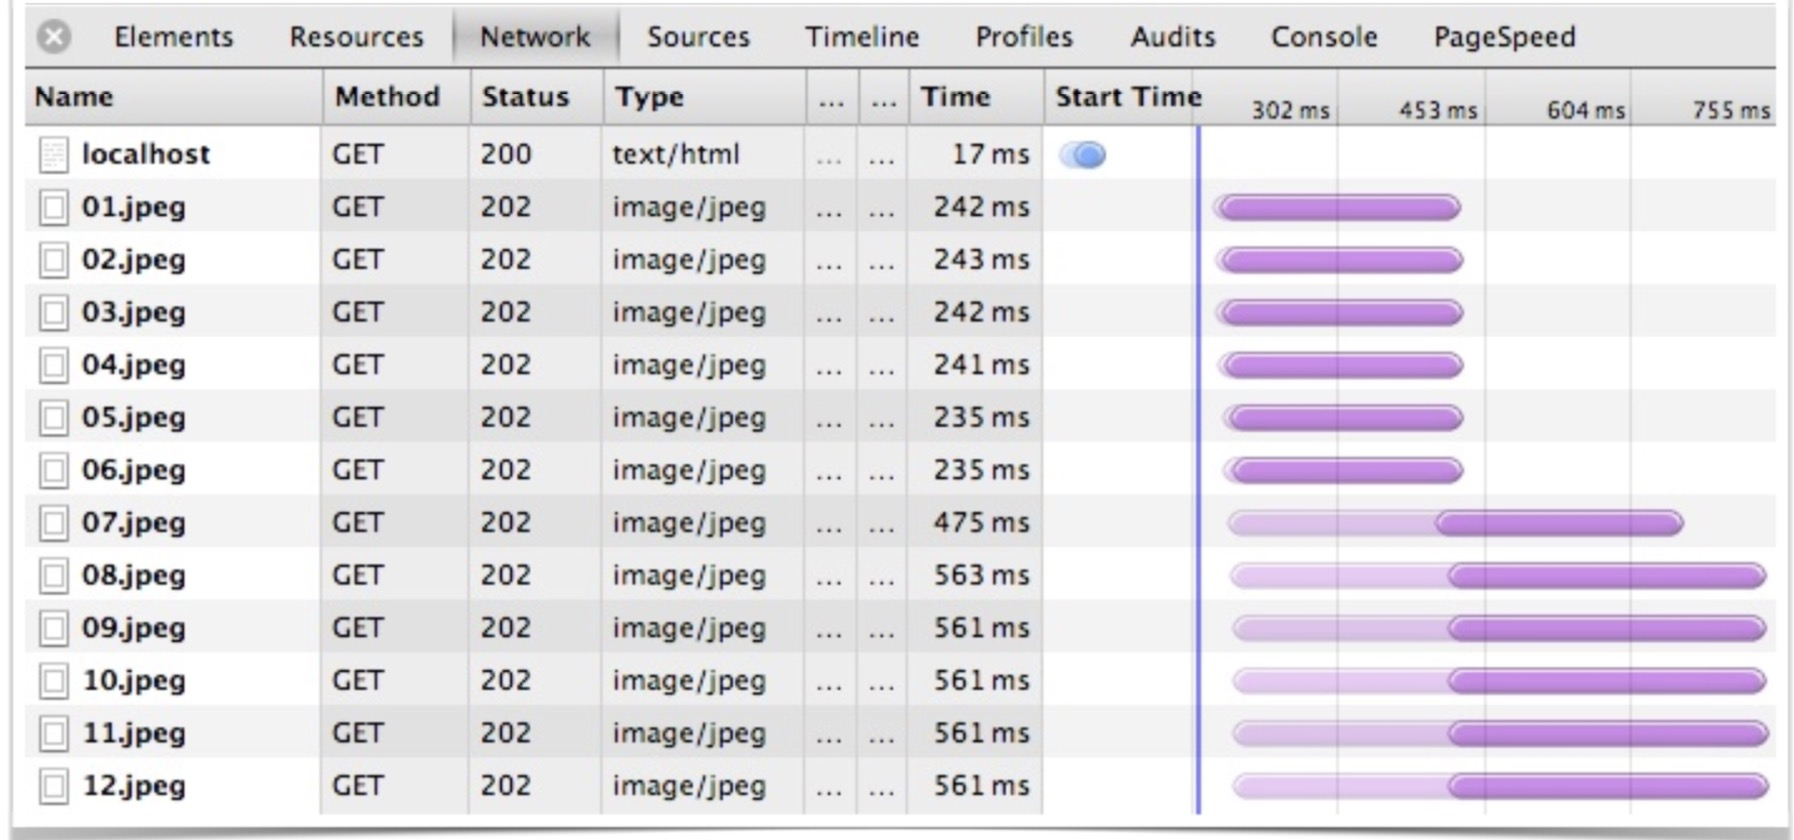
\includegraphics[scale=0.2]{Figures/web_load.jpg}
	\subsection{HTTP/2的新增特性及转换实现}
	针对上文提到的HTTP/1.1的问题,2015年IETF发布的HTTP/2协议新增了若干特性:
	\begin{itemize}
		\item 引入了流(Stream)的概念,取消了Keep-Alive而采用多路复用机制。
		\item 引入二进制分帧,将消息分割为更小的帧,并采用二进制格式进行编码。其中头(Header)会被专门封装到Headers帧中。
		\item 引入头部压缩机制,将一些常用头部用单字节表示,缩减头部大小。
	\end{itemize} \par
	这些机制解决了并发连接的问题,并在一定程度上缩减了每次HTTP传输的大小,显著提高了响应速度和TCP传输的效率\cite{de2015http}。\par 
	当然,HTTP/2还不只增加了这些特性。HTTP/2设计时还考虑到其作为一个多用途的网络通讯协议,因此
	还增加了诸如服务端主动推送这样的特性。目前现代浏览器还没有实现这些特性,暂不在本设计的考虑范围之内。
	特别需要注意的是,HTTP/2目前有H2C和H2两种实现类型\cite{belshe2015hypertext}。H2C是目前主流浏览器所实现的类型,
	该实现较为强调传输的安全性,强制通过TLS加密传输的数据。H2多用于非Web等对安全性要求较低的应用场景,例如RPC调用等。下文所讨论的均默认为H2C的实现。\par
	对于协议的处理,本网关最重要的功能就是将用户发送的HTTP/2的请求修改为HTTP/1.1的,以及将HTTP/1.1的响应修改为HTTP/2的。 
	本节讨论的就是如何对报文处理以达到我们的目的。\par 
	HTTP/2的报文格式在设计时尽可能地兼容了HTTP/1.1,请求报文基本上只需要修改头部请求的协议即可。\par 
	对于响应的报文则需要做如下操作:\par 
	\begin{itemize}
		\item 去除Keep-Alive相关的头部,包括Connection和Keep-Alive。
		\item 对头部采用HPACK算法\cite{peon2015hpack}进行压缩。
	\end{itemize}
	之后将处理的报文按照HTTP/2的二进制帧的格式写入即可。
	\subsection{HTTP/2协商机制}
	在HTTP/1.1和HTTP/2共存的环境下,浏览器和客户端要怎么样才能知道到底应该选择哪个协议来沟通?
	毕竟还有很多低版本浏览器不支持HTTP/2。本节将介绍目前主流的客户端与服务端的协商机制,这一机制
	也用在了我们设计的网关当中。\par 
	这就要谈到HTTP/1.1中的Upgrade机制,这一机制能够使得客户端和服务端之间借助已有的HTTP语法
	升级到其它协议。对于H2C的升级,正是借助Upgrade来实现的\cite{fielding2014hypertext}。\par 
	如果客户端(浏览器)支持HTTP/2,就必须通过Upgrade头部列出要升级的协议和版本,并且还要包含一个HTTP2-Settings
	的头部,示例报文如下:\\
	\fbox{%
		\parbox[c][88pt][t]{420pt} {
		GET / HTTP/1.1 \\
		Host: www.example.com \\
		Connection: Upgrade, HTTP2-Settings \\
		Upgrade: h2c \\
		HTTP2-Settings: <base64url encoding of HTTP/2 SETTINGS payload> \\
		}%
	} \par
	如果服务器不支持HTTP/2便会忽略Upgrade头部,直接响应HTTP/1.1的报文。示例报文如下:\\
	\fbox{%
		\parbox[c][68pt][t]{420pt} {
		HTTP/1.1 200 OK\\
		Content-Length: 1234\\
		Content-Type: text/html\\
		...
		}%
	} \par
	反之,如果服务端支持HTTP/2,那就可以回应101状态码及其对应头部,并且在响应正文中直接传送
	HTTP/2的二进制帧。示例报文如下:\\
	\fbox{%
		\parbox[c][68pt][t]{420pt} {
		HTTP/1.1 101 Switching Protocols\\
		Connection: Upgrade\\
		Upgrade: h2c\\
		HTTP/2 connection...
		}%
	} \par
	以上就完成了客户端和服务端协商使用哪种协议的流程。该流程能够确保在协议不冲突的情况下尽可能
	地强制客户端和服务端通过HTTP/2进行通信。
	\subsection{WebSocket支持}
	WebSocket协议本身不是HTTP标准的一部分。HTTP/1.x协议的重要缺陷之一就是难以进行交互式通信,
	对于实时聊天和长轮询等功能只能通过开启大量HTTP请求来解决。为了解决这个问题,
	IETF专门设计了一个新的协议WebSocket用于交互式通信的场景,其协议标准在RFC 6455中规定\cite{fette2011websocket}。\par
	3.2节中提到,HTTP/2引入了服务端推送机制,如果能够在应用开发中使用这一机制,那么是能够
	有效替代WebSocket协议的。但目前不论是客户端还是我们所要升级的目标服务,都是采用WebSocket协议。
	因此我们要在网关中加入对反向代理WebSocket协议的支持。这需要我们分析WebSocket协议的建立与
	传输流程,并针对性地设计反向代理的方法。\par
	在HTTP网关的部分,我们要解决的问题是客户端与服务端之间如何从HTTP协议切换到WebSocket协议。3.3节中
	提到的HTTP/1.1的Upgrade机制同样适用于此处。需要注意的是,HTTP/2不提供Upgrade机制,因此下文
	所讨论的依然是基于HTTP/1.1展开。\par
	通过Upgrade机制升级WebSocket协议的示例报文如下:\\ 
	\fbox{%
		\parbox[c][105pt][t]{420pt} {
			GET /chat HTTP/1.1 \\
			Host: www.example.com \\
			Upgrade: websocket \\
			Connection: Upgrade \\
			Sec-WebSocket-Key: x3JJHMbDL1EzLkh9GBhXDw== \\
			Sec-WebSocket-Protocol: chat\\
		}%
	} \par
	Sec-WebSocket-Key是一个客户端随机生成的值,它用于唯一标识一个WebSocket连接。
    Sec-WebSocket-Protocol 表示最终使用的协议。	
	如果服务端支持WebSocket的协议的话,将会返回HTTP 101响应,示例报文如下:\\
	\fbox{%
		\parbox[c][68pt][t]{420pt} {
		HTTP/1.1 101 Switching Switching Protocols\\
		Connection: Upgrade\\
		Upgrade: websocket\\
		...
		}
	} \par
	至此,HTTP网关本身负责的HTTP协议的部分已经结束了。接下来数据帧的格式直接交给源站处理即可,我们的网关只需开辟一条从客户端到源站的
	TCP连接即可完成源站与客户端接下来的WebSocket协议通信。
	\subsection{HTTPS支持}
	HTTPS(Hypertext Transfer Protocol Secure)是以安全为目标的HTTP通道。
	它通过多种对称加密和非对称加密算法对HTTP传输内容进行加密。\par 
	HTTP/2协议本身并不要求是加密的,但目前所有的浏览器都强制要求HTTP/2协议传输的数据是HTTPS加密的。
	在具体实现中,我们可以认为浏览器中HTTP/2是在应用层中的TLS(Transport Layner Security)\cite{rescorla2000http}
	层之上进行传输的,HTTP/2和TLS共同构成了HTTPS。\par 
	为了使得我们的网关能够支持现代浏览器,在本设计中加入HTTPS支持。在TCP传输时增加TLS操作,加密数据。本设计是通过Go语言中crypto库
	中已经实现的TLSv1.2标准进行加密的,目前包括Chrome,FireFox在内的主流浏览器最近的几个大版本均支持这一标准。
	在运行程序之前,用户也需要先做好HTTPS证书相关的配置。\par

	%-- 第四章
	\begin{spacing}{2}
		\section{IPv4和IPv6双栈环境下反向代理功能的实现}
	\end{spacing}
	设计的网关是在反向代理的过程中完成前一章所讨论的对HTTP/2协议的处理,本章讨论了反向代理的实现和
	其如何在IPv6和IPv4双栈环境下工作。并设计了负载均衡策略以满足高并发环境下的业务需求。
	
	\subsection{反向代理的实现}
	前面提到,本网关通过反向代理功能升级HTTP服务。反向代理本身的功能十分简单,服务器根据客户端的请求,从其关系的一组或多组提供HTTP服务的源站服务器上获取数据,
	然后再将这些数据返回给客户端。客户端只会得知反向代理服务器的IP地址,而不知道在代理服务器后面的服务器集群的存在。 \par 
	前一章提到的HTTP/1.1报文转换为HTTP/2报文就是在反向代理过程中实现的。反向代理服务器收到客户端的HTTP请求后,将报文
	修改为HTTP/1.1格式的,发送到源站服务器;源站服务器响应后再将源站返回的HTTP/1.1的报文修改为HTTP/2格式的,返回给客户端。
	当然,这其中还需要注意HTTP超时和源站崩溃的问题,设计中通过上文提到的Context监听这种异常情况。对于出现异常情况,根据HTTP状态码的定义响应对应的状态码即可。流程图如图所示:\par
	\begin{center}
	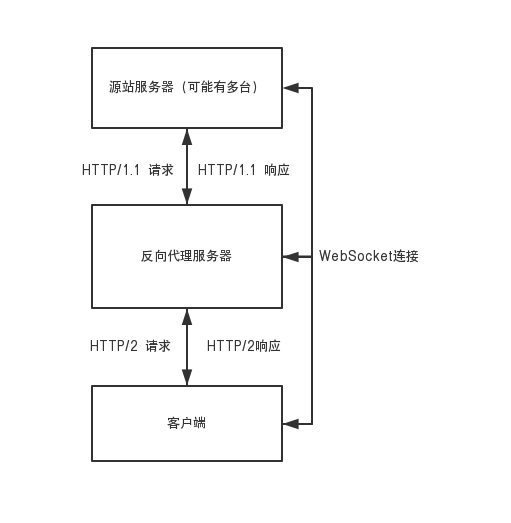
\includegraphics[scale=0.56]{Figures/reverse_proxy.png}
	\end{center}
	\subsection{负载均衡策略}
	高并发环境下,为了减少由于访问量过多引起服务器系统崩溃的情况,我们常常需要对源站进行动态扩容。这其中最简单的方式就是横向扩容,
	通过多个相互独立的服务器组成一个集群服务器系统,从而较好地应对高负载情况。\par 
	为了达到这一目的,我们设计的网关需要提供负载均衡的功能。即把转发的HTTP请求分摊到
	不同的源站进行处理,降低单一机器的负载压力\cite{夏斌2014云服务平台负载均衡器的网络设计与实践}。为了尽可能地利用有限的服务器资源,我们的负载均衡
	策略均要求具有一定的平滑性和均衡性。\par
	本设计针对两种较常出现的业务场景,根据目前较为成熟的算法,设计了两种不同的负载均衡策略。一种是业务简单且对负载均衡性能要求极高的场景,
	采用加权轮询算法实现;一种是存在HTTP会话的场景,即用户可能需要通过Cookie等手段与同一台源站服务器保持一段时间
	的会话。这时如果将同一用户的不同HTTP请求发送到不同服务器会导致我们的业务流程无法正常完成。
	这时采用一致性哈希算法,将同一IP来源的用户的请求发送到同一台服务器,并使得请求尽可能均摊到不同服务器上,
	且在出现节点故障时能够以最小的损耗将请求迁移到其它机器。本节讨论了这两种策略的具体实现。\par 
	
	\subsubsection{加权轮询算法(Weighted Round Robin)}
	轮询(Poll)本身是一种非常简单的算法。假设有我们有三台源站服务器ServerA, ServerB,ServerC,
	那么我们可以生成一个序列\{ServerA, ServerB, ServerC\},对这个序列进行不断地遍历来获得轮询结果。\par 
	当我们需要的源站服务器具有不同的权重时,情况就会比较复杂了。假设对于上面三台服务器,分别具有3,2,1大小的权重,
	那么我们通过轮询算法生成的序列就是\{ServerA, ServerA, ServerA, ServerB, ServerB, ServerA \}。
	对这个序列遍历获取轮询结果确实能达到一定的负载均衡的效果,但这种负载均衡策略不具有平滑性和均衡性,
	在不同的时间不同机器的负载是有很大差别的。\par 
	Nginx对上述的加权轮询算法进行了改进,设计了一种平滑的加权轮询算法\cite{wrr}。本设计
	使用了与Nginx中一致的加权轮询策略。\par 
	该加权轮询策略首先需要给每个源站服务器分配三个权重。weight 是每个源站服务器恒定不变的负载权重;
	effective weight是实际有效权重,一开始与weight大小相同,用于根据实际情况动态调整的权重;current weight 是一个在
	运行过程中动态调整的值。该策略的具体步骤如下:
	\begin{itemize}
		\item 对每个请求,遍历所有源站服务器,对每个源站服务器的current weight 的值自增 effective weight 值的大小。同时累加所有源站的effective weight,保存为total。
		\item 从所有源站服务器中选出current weight 最大的一个,作为本次命中的源站服务器。
		\item 对本次选中的源站服务器,对其current weight 的值自减 total的值。
	\end{itemize}
	\par
	使用这一策略对上文提到的权重分别为3, 2 , 1的三个源站服务器,其生成的轮询序列示例如下:\\
	\begin{tabular}{|c|c|c|c|} 
		\hline
		请求序号 & 选择前的current weight & 选中源站服务器 & 选择后的current weight  \\ \hline
		1 & \{3, 2, 1\} & ServerA & \{-3, 2, 1\} \\ \hline
		2 & \{0, 4, 2\} & ServerB & \{0, -2, 2\} \\ \hline
		3 & \{3, 0, 3\} & ServerA & \{-3, 0, 3\} \\ \hline
		4 & \{0, 2, 4\} & ServerC & \{0, 2, -2\} \\ \hline
		5 & \{3, 4, -1\} & ServerB & \{3, -2, -1\} \\ \hline
		6 & \{6, 0, 0\}  & ServerA & \{0, 0, 0 \} \\
		\hline
	\end{tabular}
	\par
	可以看出该策略生成的序列较为平滑,且满足负载均衡中均衡分布的要求。6次轮询过后current weight回到了{0, 0, 0},意味着
	若继续执行该算法,将不断生成相同的序列。


	\subsubsection{一致性哈希算法(Consistenting Hashing)}
	一致性哈希算法由美国麻省理工学院在哈希算法的基础上提出\cite{karger1997consistent},
	它的目标是解决动态系统中均衡分布的问题。与直接采用一般哈希算法取模的做法比起来,该算法具有更强的平衡性、单调性、平滑性和分散性,
	适用于因特网中的热点问题,同样也适合本设计中的负载均衡策略。本设计就以用户IP作为Hash Key,通过一致性哈希算法解决本设计中特定场景的负载均衡问题。\par 
	本设计根据实际需求实现了如下描述的一致性哈希算法中的六个步骤,实现了取模、映射、删除服务器节点的功能,达到了均衡和单调的要求。\par
	\paragraph{构造环形哈希表}
	首先创建一个32位大小的key值,然后将这个数据空间首尾相连,
	形成一个环形哈希环。
	\paragraph{将请求映射到哈希环}
	将用户请求时的IP地址作为字符串处理,采用一般哈希算法,将这个字符串计算得到一个32位的值,对于请求ReqN我们得到KeyN,
	然后映射到哈希环上。本例中采用的是Go语言内置库crypto中实现的MD5算法。
	\paragraph{将源站服务器映射到哈希环}
	如同上一步骤一样,通过一般哈希函数,以服务器IP作为Hash Key将服务器也处理成一个32位的值,映射到同一个哈希环中,对于ServerM我们可以得到一个KeyM。
	增加和减少源站服务器时,在环形哈希环上作适当的增删。
	\paragraph{将请求映射到源站服务器}
	顺着哈希环的顺时针方向,从请求Key1开始查找,一直到遇到第一台服务器Server1为止,将该请求
	Key1映射到Server1上。由于这两者我们计算出来的哈希函数是固定的,因此它们的映射关系是唯一的,可以保证同一IP的用户会一直映射到同一台源站服务器上。
	以此类推,对应映射ReqN到ServerM上,一直到所有的请求和服务器映射关系建立完成。
	\paragraph{动态增减源站服务器}
	一致性哈希算法的重要特点之一就是支持对源站服务器的动态增减,使得我们在特定场景下能够以较少
	的损耗动态迁移源站服务器。当要增加服务器Server(M+1)时,通过一般哈希算法得出Key(M+1),
	该Key数值介于原来的两台服务器的值之间,虽然新增了服务器,但只需要重新映射Key(M+1)逆时针
	出发遇到的第一台服务器Key之间的请求,其余的接入请求和服务器保持原有的映射关系不变。
	移除服务器KeyB时,同理,受影响的也只是逆时针出发达到的第一台服务器KeyA的接入请求,也只需要
	将Key1和新服务器进行重新映射即可,如图所示。\\
	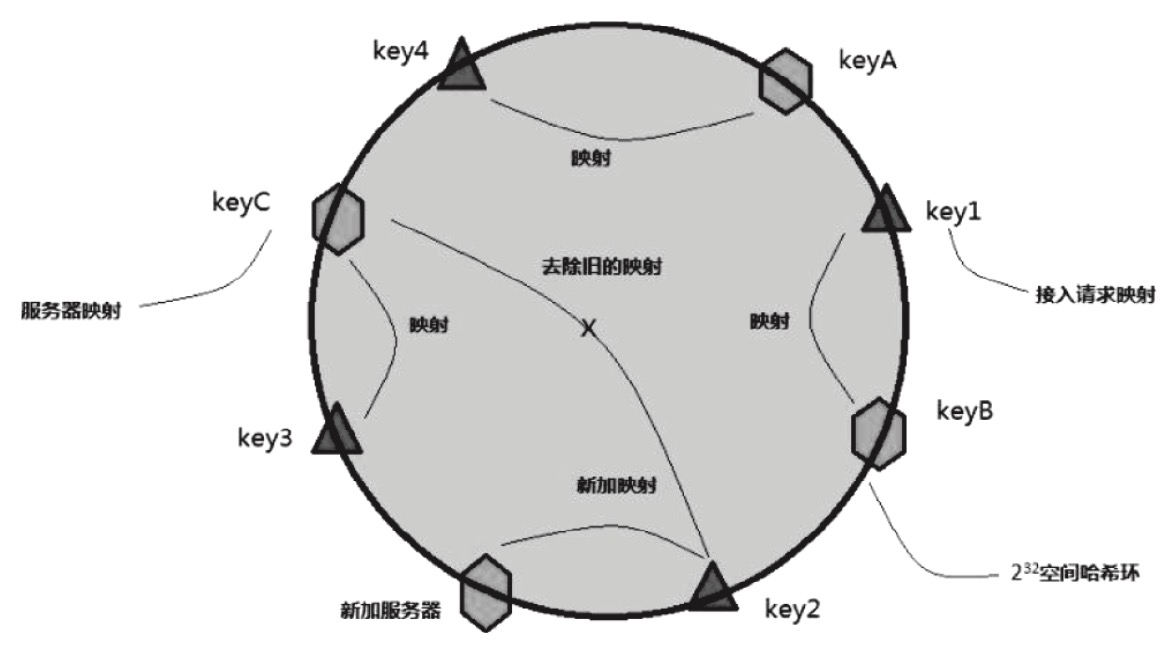
\includegraphics[scale=0.36]{Figures/hash_circle.jpg}

	\par 
	通过上述六个步骤,即可完成基于一致性哈希算法的负载均衡策略。

	\subsection{IPv6环境下工作}
	IPv6是网际协议的最新版本,用作互联网的网络层协议。用它来取代IPv4主要是为了解决IPv4地址枯竭问题,
	同时它也在其他方面对于IPv4有许多改进。 \par 
	在网络上,数据以分组的形式传输。IPv6定义了一种新的分组格式,目的是为了最小化路由器处理的消息标头。
	由于IPv4消息和IPv6消息标头有很大不同,因此这两种协议无法互操作。但是在大多数情况下,IPv6仅仅是对IPv4的一种保守扩展。
	除了嵌入了互联网地址的那些应用协议(如FTP和NTPv3,新地址格式可能会与当前协议的语法冲突)以外,
	大多数传输层和应用层协议几乎不怎么需要修改就可以在IPv6上运行\cite{伍佑明2009ipv6}。 \par 
	我们开发的网关是在应用层开发的,因此对于IPv6不需要过多的处理。事实上,Go的内置的net库所有的
	操作均已支持对IPv6地址的处理。只需要让设计的网关支持在多Host和多端口监听即可。

	%-- 第五章
	\begin{spacing}{2}
		\section{性能分析}
	\end{spacing}

	本章对设计的网关模拟高并发场景,进行系统测试。主要分两部分进行测试。一部分是压力测试,
	测试了系统极吞吐量和响应时间。另一部分是
	对网关内各个调用开销的分析,使用了火焰图进行可视化分析。\par 
	本次测试使用的计算机的基本配置如下:\par 
	\begin{itemize}
		\item CPU: Intel(R) Xeon(R) CPU E5-2660 v3
		\item 物理核数:8
		\item 逻辑核数:8
		\item 内存:32G
		\item 操作系统:Ubuntu 17.10 artful, Linux Kernel 4.13.0-46-generic
	\end{itemize}
	\subsection{压力测试}
	压力测试使用的工具是nghttp2,这是一个专门为HTTP/2服务端应用设计的开源压力测试工具。测试方法和结果如下:\par 
	\begin{enumerate}
	\item 源站放在服务器本地,源站提供简单的静态页面的访问,单个资源大小均小于20KB。nghttp2随机访问任意URL。nghttp2使用10个线程进行请求,共计请求一万次。
	总计在2.85s完成了所有请求,平均每秒完成3507.9个请求,失败请求数为0。其它统计数据如下:
	\begin{center}
	\begin{tabular}{|c|c|c|c|} 
		\hline
		 \ & Min & Max & Mean  \\ \hline
		time for request & 1.15ms  & 4.13ms & 2.83ms \\ \hline
		time for connect & 3.54ms & 11.27ms & 8.16ms \\ \hline
		time to 1st byte & 9.43ms  & 13.07ms & 10.39ms \\
		\hline
	\end{tabular}
	\end{center}
	\item 源站放置在服务器本地,源站提供几个4GB以上的大文件的静态资源访问。开启十个线程GET访问的资源。平均流量大小为124.78M/s。
	但关闭HTTPS支持之后则能够达到2000M/s以上,不难发现流量瓶颈主要来源于网关加密资源带来的开销。
	\item 源站放置在远程服务器上,模拟线上环境,源站返回响应存在一定延时。源站的资源与测试1相同,但是平均有200ms左右的延时且较不稳定。测试方法与
	测试1也相同。总计在296.02s完成了所有请求,平均每秒完成337.5个请求,失败请求数为2(发生了超时,响应500状态码)。
	反向代理产生的延迟和直接请求源站并没有显著差别,反向代理产生的损耗可以忽略不计,统计数据如下:
	\begin{center}
		\begin{tabular}{|c|c|c|c|} 
			\hline
			 \ & Min & Max & Mean  \\ \hline
			time for request & 76.23ms  & 1566.30ms & 218.10ms \\ \hline
			time for connect & 17.52ms & 19.17ms & 18.39ms \\ \hline
			time to 1st byte & 115.38ms  & 619.48ms & 234.98ms \\
			\hline
		\end{tabular}
		\end{center}
	\end{enumerate}
	\par
	从上述数据可以看出,本网关具有较强的并发性能,且能够高效处理存在I/O阻塞的异步事件。

	\subsection{火焰图}
	火焰图是一种用来分析程序内部调用开销的方法\cite{gregg2017visualizing}。它通过可视化地展示各个事件占用的CPU时间比例
	来帮助我们分析程序的性能瓶颈,能够帮助我们捕捉到压力测试下可能发现不了的问题。\par
	Go语言内置了pprof包用于监测性能,配合一个使用Perl语言编写的开源火焰图可视化工具FlameGraph即可对运行中的程序绘制火焰图。
	测试时通过nghttp2工具模拟了线上环境,对本网关绘制的火焰图如下:\\
	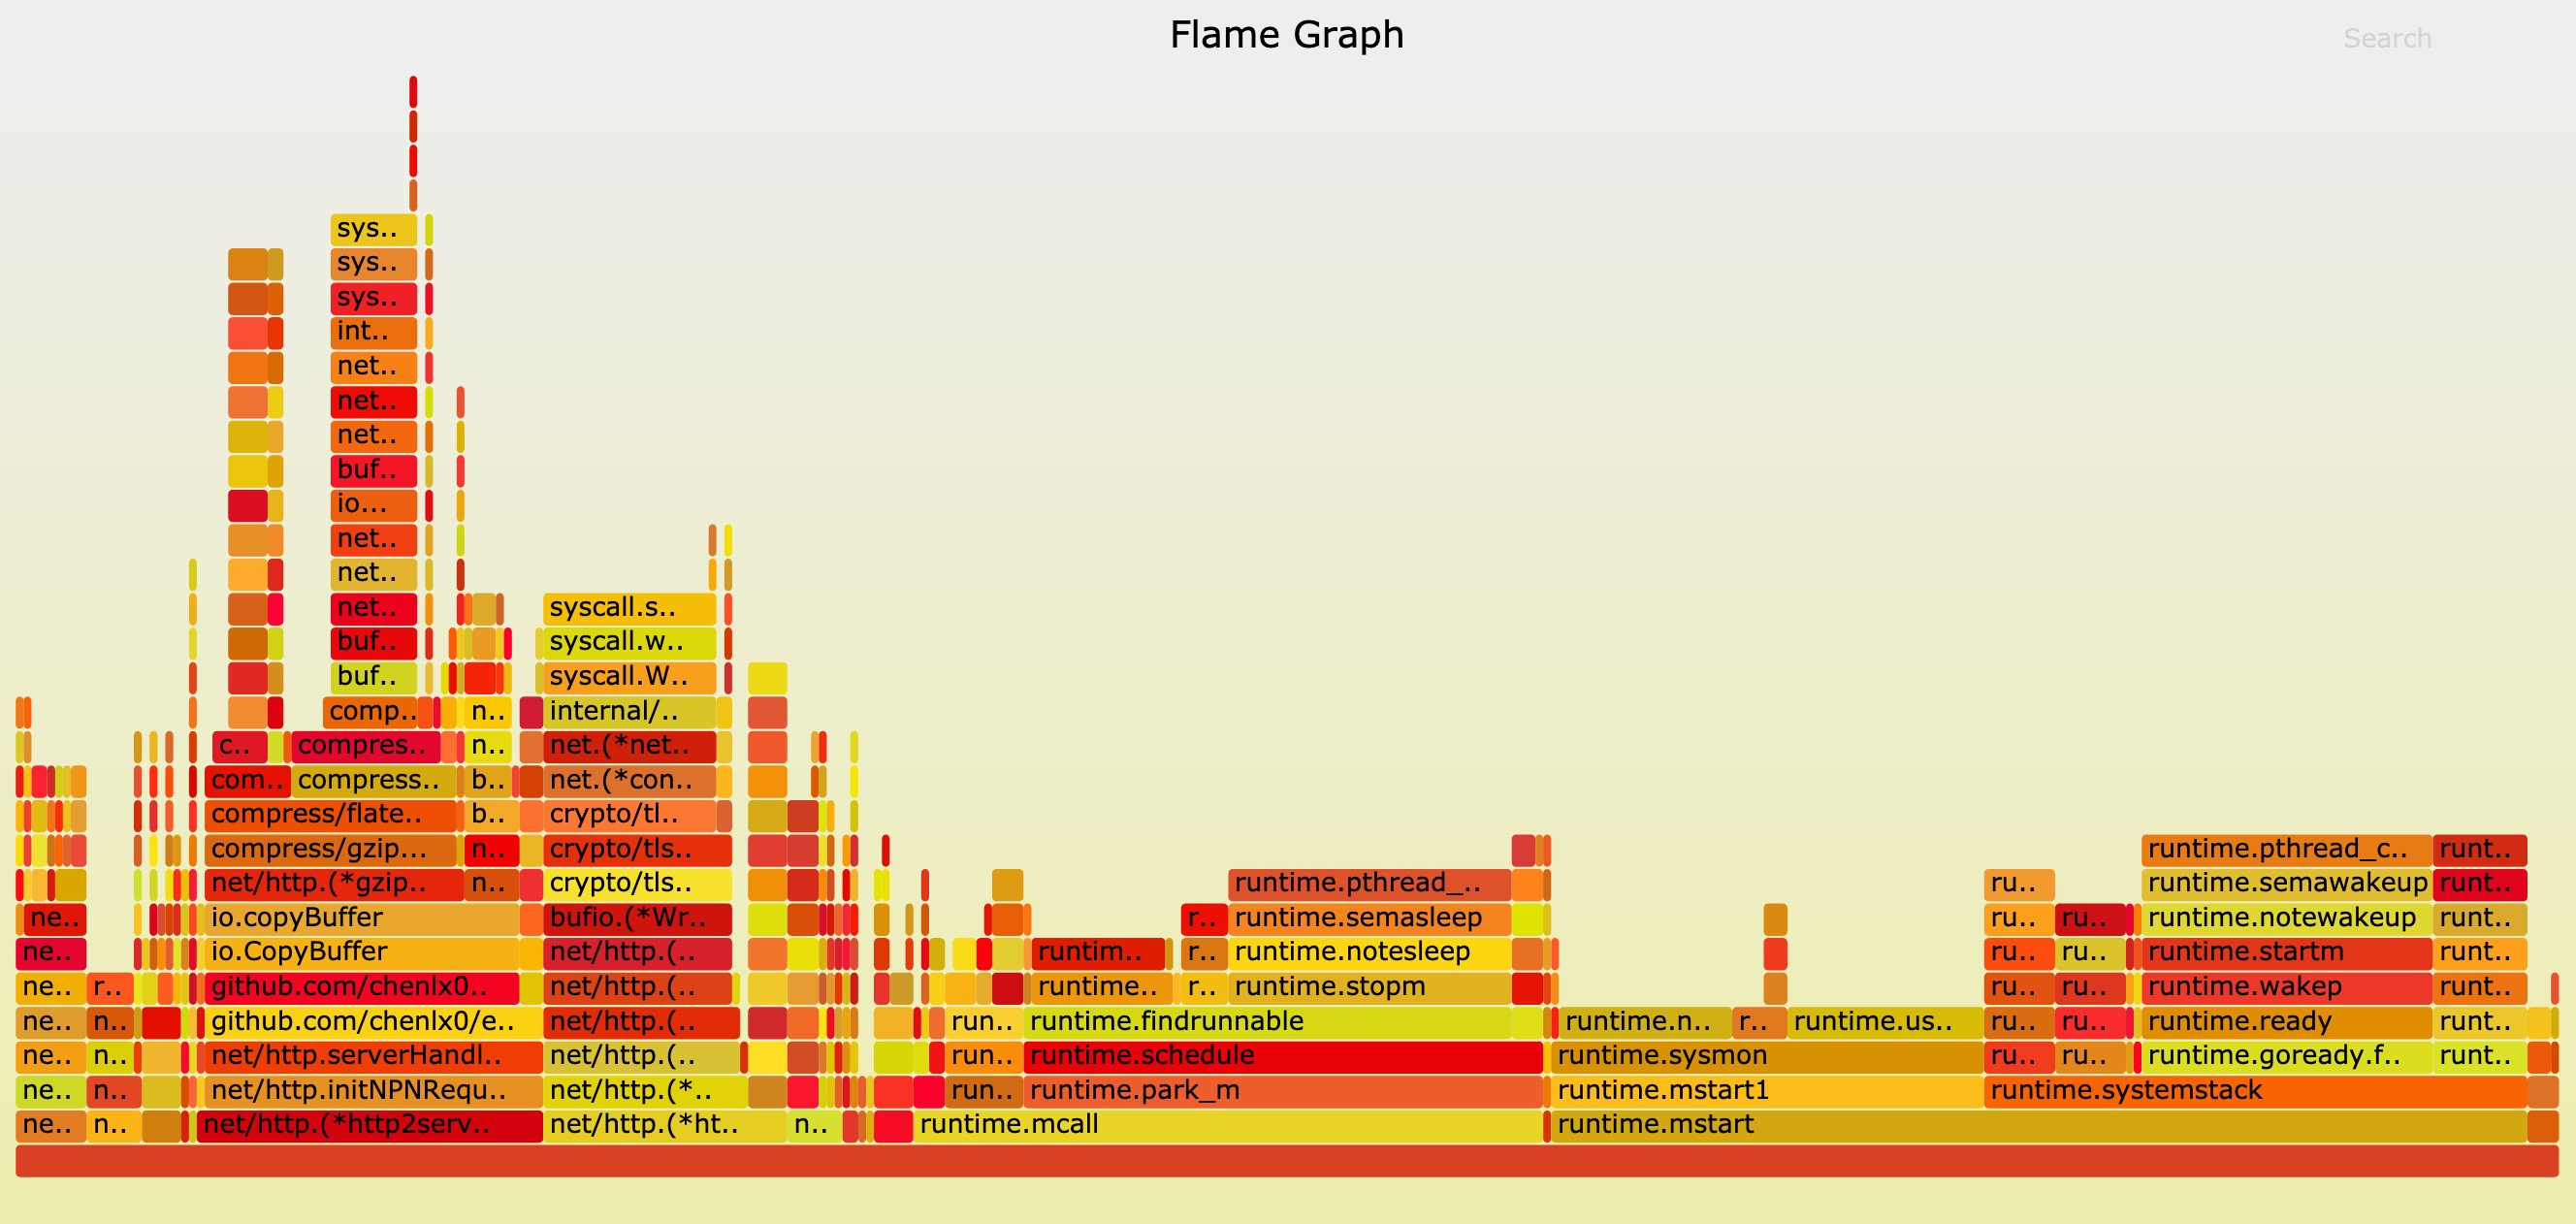
\includegraphics[scale=0.158]{Figures/flame_graph_simple.jpg}
	\par 
	从图中可以看出,各调用之间分布较为均匀。runtime开头的调用多为Go底层对协程上下文切换等操作的
	调用,除了这之外,占用资源较多的调用为网关监听端口进行数据拷贝的调用和HTTP/2数据帧写入和加密的调用。
	总体来说没有哪一个调用过多占用了CPU资源,调用比例较为合理,符合本设计的最初的设想。

	%-- 第六章
	\begin{spacing}{2}
		\section{总结与展望}
	\end{spacing}
	 本文设计了一个基于IPv6和IPv4双栈环境的HTTP/2过渡应用, 能够帮助用户以较低的成本
	 将原有的IPv4环境下HTTP/1.1的应用通过本网关以反向代理技术升级支持IPv6和HTTP/2协议,
	 并且提供了负载均衡技术,能够帮助原有的应用进行横向扩容,且具有较好的并发性能。适合作为
	 当前多种协议共存环境下过渡升级新协议的服务端应用。\par 
	 但本文设计的这一应用依然有需要改进的地方:
	 \begin{itemize}
		\item 直接使用Go内置已经实现的TLSv1.2加密方法固然方便,但效率较低,在大流量情况下容易出现瓶颈。
		最好能够自己实现最新的TLSv1.3加密方法,能够大幅度提高加密效率。
		\item 缺少对源站的实时监控机制,源站崩溃时不容易发现问题。
		\item 缺少对客户端请求的过滤机制,遭遇恶意请求容易崩溃。
	 \end{itemize}
	
	%---------------------------------------------  致谢  ---------------------------------------------
	\begin{spacing}{2}
		\section*{致谢}
	\end{spacing}
	\phantomsection
	\addcontentsline{toc}{section}{致谢}
	大学四年转瞬即逝,四年以来在中国地质大学(武汉),结交了许多老师和同学,
	得到了很多帮助,让我从一个懵懂的高中生成长为了一个合格的本科生。\par 
	感谢我的导师张峰老师。张老师是一位治学严谨,和蔼可亲的导师,从学习内容到人生疑惑,
	张老师都能给我耐心的指导。同时感谢中国地质大学(武汉)网络中心和帅赟老师,
	给了我在大学生涯中以大量的计算机软件开发的相关实践机会、资源和指导。\par 
	感谢中国地质大学(武汉)计算机学院,给了我们良好的学习和生活环境,感谢每一位
	辛勤付出的老师和职工。\par
	感谢大学期间实习的两个单位,一个是大三暑假实习的武汉微派网络有限公司,
	让我接触到了Go语言及相关的技术;另一个是毕业实习的单位,网易(杭州)网络有限公司网络管理部CDN组。使我了解了相关领域
	业界的发展方向,提高了自己的相关技能。\par
	最后感谢我的父母,是他们让我有一个温暖的家庭,让我无忧无虑地完成了十几年的学业。
	感谢大学期间帮助我的各位同学,特别是信工学院08级的学长吴永城,无私地帮助和引导我,
	带我走进了计算机行业的大门。还有姜瑞,夏丁,郑健等同学,感谢你们与我走过了一个
	最有价值的本科生生涯。
	
	
	\clearpage
	%---------------------------------------------参考文献---------------------------------------------
	
	\bibliography{Bibs/mybib}
	\phantomsection
	\addcontentsline{toc}{section}{参考文献}
	
\end{document}